\documentclass{emulateapj}
%\documentclass[12pt,preprint]{aastex}

\usepackage{graphicx}
\usepackage{float}
\usepackage{amsmath}
\usepackage{epsfig,floatflt}
\setcitestyle{square}
\usepackage{subfig}


\DeclareMathAlphabet{\mathcal}{OMS}{cmsy}{m}{n}
\SetMathAlphabet{\mathcal}{bold}{OMS}{cmsy}{b}{n}


\begin{document}

\title{Project 2}

\author{Stig-Nicolai Foyn, Christer Dreierstad}

\email{stignicf@student.matnat.uio.no, chrisdre@student.matnat.uio.no}

\altaffiltext{1}{Institute of Physics, University of
  Oslo, P.O.\ Box 1029 Blindern, N-0315 Oslo, Norway}


\begin{abstract}

\end{abstract}
\keywords{classical physics --- quantum mechanics --- electromagnetism --- methods: numerical, scaling of equations, Jacobi's method}

\section{Introduction}
\label{sec:introduction}
In this paper we will show how to transform problems such that it can be solved as an eigenvalue problem by Jacobi's method. We will start by considering a beam fastened in both ends with a force F acting on it, and further apply the method to a quantum mechanical system of an electron in a harmonic oscillator potential. Lastly we will be extending the method to a two electron system in a harmonic oscillator potential where the electrons interact via Coulomb repulsion. By scaling the differential equation that describes the systems above, we obtain an equation that can be solved as an eigenvalue problem. The scaled equation is then discretized and set up as a matrix, which method  was discussed in our previous paper\cite{1}, which allows us to apply Jacobi's method to solve the problem. We will be comparing the CPU time of Jacobi's method to Armadillo's method for solving an eigenvalue problem. Also comparing the calculated eigenvalues of Jacobi's method with Armadillo's function and the analytically calculated eigenvalues. When we extend the problem to a quantum mechanical one, the matrix no longer has identical values along the diagonal (i.e. no longer a Toeplitz matrix) as the harmonic osillator potential, and the Coulomb repulsion, is not constant as the electrons move in the system. 


\section{Method}
\label{sec:method}
The method presented will show how to solve an eigenvalue problem using Jacobi's method and that by scaling the equations for a given problem, one can transform the problem to an eigenvalue problem on a matrix form with known analytical eigenpairs. The first problem is a classical one involving a beam fastened in both ends. Further the method is applied to a quantum mechanical three dimensional quantum dot problem, starting with one electron and moving over to a problem with two electrons.

\subsection{Jacobi's method for solving an eigenvalue problem}
Solving the eigenvalue problem with Jacobi's method means solving an equation on the form
%
\begin{gather}\label{eq:B=SAS}
    \bold{S}^T\bold{A}\bold{S} = \bold{B},
\end{gather}
%
where $\bold{S}$ is an orthogonal matrix, so it has the property $\bold{S}^{-1} = \bold{S}^T$. The resulting matrix $\bold{B}$ will consist of the eigenvalues along the diagonal. The matrix $\bold{S}$ is such that the elements along the diagonal are 1, and zero elsewhere, except four elements which are such that their position are decided by the largest element of the off-diagonal of $\bold{A}$. The largest element of $\bold{A}$ is found at a position $(k,l)$, and these indices are used to define the position of the mentioned four elements of $\bold{S}$, which are such that $s_{kk} = s_{ll} = \cos\theta$ and $s_{kl} = -s_{lk} = -\sin\theta$. This is considered as a rotation of an angle $\theta$ in the n-dimensional Euclidean space. When solving \eqref{eq:B=SAS} the resulting equations to solve are
%
\begin{align*}
    &b_{ii} = a_{ii}, i \neq k, i \neq l \\
    &b_{ik} = a_{ik}c - a_{il}s, i\neq k, i\neq l \\
    &b_{il} = a_{il}c + a_{ik}s, i \neq k, i\neq l \\
    &b_{kk} = a_{kk} c^2 - 2a_{kl}cs+ a_{ll}s^2 \\
    &b_{ll} = a_{ll} c^2 + 2a_{kl}cs a_{kk}s^2 \\
    &b_{kl} = \left(a_{kk} - a_{ll}\right)cs + a_{kl}\left(c^2 - s^2\right),
\end{align*}
where $c = \cos\theta$ and $s = \sin\theta$. The main goal is to reduce the off-diagonal elements of $\bold{A}$ to zero in such a way that $\bold{B}$ has the eigenvalues along the diagonal, the reduction of the elements is done by choosing the angle $\theta$. We make a requirement that the off-diagonal elements of $\bold{B}$ is zero;
%
\begin{align*}
    b_{kl} &= 0 = \left(a_{kk} - a_{ll}\right)cs + a_{kl} \left(c^2 - s^2\right),
\end{align*}
%
which can then be written as
%
\begin{gather*}
    \frac{\left(a_{ll} - a_{kk}\right)}{a_{kl}}cs = \left(c^2 - s^2\right).
\end{gather*}
%
Defining $\tau = \left(a_{ll} - a_{kk}\right)/2a_{kl}$ and $\tan\theta = t = s/c$, and multiplying the equation above by $1/c^2$ we obtain a quadratic equation 
%
\begin{gather*}
    t^2 + 2\tau t - 1 = 0,
\end{gather*}
%
which is used to define the best fit $\theta$ to reduce the off-diagonal elements of $\bold{A}$. The solution to the quadratic equation is $t = -\tau \pm \sqrt{1 + \tau^2}$. If $\tau$ becomes large, the numerical accuracy will drop and $t \approx -\tau \pm \tau$. By the following transformation
%
\begin{align*}
    t_{\pm} &= -\tau \pm \sqrt{1+\tau^2}\left(\frac{\tau \pm \sqrt{1+\tau^2}}{\tau \pm \sqrt{1+\tau^2}}\right) \\
    &= \frac{-\tau^2 + \left(1 + \tau^2\right)}{\tau \pm \sqrt{1 + \tau^2}} = \frac{1}{\tau \pm \sqrt{1+\tau^2}}.
\end{align*}
%
and by splitting the equation such that when $\tau < 0$ we choose the negative sign in front of the square root the aforementioned issue is avoided. The final equations for t are
%
\begin{align*}
    t_+ = \frac{1}{\tau + \sqrt{1 + \tau^2}}, \tau \geq 0 \\
    t_- = \frac{1}{\tau - \sqrt{1 + \tau^2}}, \tau < 0
\end{align*}
%
From the definition of $t = \tan\theta$, s can be expressed as
%
\begin{align*}
    s = \sin\theta = \tan\theta \cos\theta = tc,
\end{align*}
and c can be expressed as
\begin{align*}
    c &= \cos\theta = \frac{\cos\theta}{\sqrt{\cos^2\theta + \sin^2\theta}} = \frac{1}{\sqrt{1 + \tan^2\theta}}  = \frac{1}{\sqrt{1 + t^2}}.
\end{align*}

 
\subsubsection{Numerical implementation}
When implementing Jacobi's method numerically, $\bold{B}$ is not explicitly created, instead the elements of $\bold{A}$ are changed during each iteration. This allows the program to run with large matrices (large n), without taking up more memory thasn needed. This means the left hand side of the six previous equations are changed so that they are valid for the elements of $\bold{A}$ instead of $\bold{B}$, meaning $b_{ii} \rightarrow a_{ii}$, $b_{ik} \rightarrow a_{ik}$ and so forth.

///EIGENVECTORS////

\subsection{Buckling beam}
Considering a beam that is fastened in both ends which moves up and down when a force F is exerted on it can be described by a differential equation
%
\begin{gather}\label{eq:du2/dx2}
    R \frac{d^2 u(x)}{dx^2} = -Fu(x),
\end{gather}
%
where $u(x)$ is the displacement of the beam in the y-direction and $R$ is a constant that is defined by the properties of the beam, such as the rigidity. Since the beam, with length L, is fastened in both ends, the displacement at the end points $u(0) = u(L) = 0$, so we have Dirichlet boundary condition as in the previous paper \cite{1}, and the sum of outer forces exerted on the beam is zero. Introducing the dimensionless variable $\rho = x/L \Rightarrow x = \rho L$, where $\rho \in [0,1]$. Introducing this into Eq. \eqref{eq:du2/dx2} gives
%
\begin{gather*}
    \frac{R}{L}\frac{d^2 u(\rho)}{d\rho^2} = - FLu(\rho)
    \Rightarrow \frac{d^2 u(\rho)}{d\rho^2} = -\frac{FL^2}{R}u(\rho).
\end{gather*}
%
Substituting $\lambda = FL^2/R$ transforms the problem to an eigenvalue problem, with discretized $\lambda$'s as eigenvalues with corresponding eigenvectors. The methods presented in the previous paper regarding the solution of a differential equation will be applied to this problem. The left hand size of the equation to solve,
%
\begin{gather}\label{eq:du/dx=lambda}
    \frac{d^2 u(\rho)}{dx^2} = -\lambda u(\rho)
\end{gather}
%
can be approximated as
%
\begin{gather*}
    \frac{d^2 u(\rho)}{dx^2} = \frac{u(\rho + h) - 2u(\rho) + u(\rho - h)}{h^2} +  \mathcal{O}(h^2),
\end{gather*}
%
where the step size $h = \left(\rho_{max} - \rho_{min}\right)/n$, which is the total length of the beam divided by the resolution of the calculations n. The maximum and minimum value of the dimensionless length variable $\rho$ is at the end points of the beam, such that $\rho_{max} = 1$ and $\rho_{min} = 0$. Following the method from the previous paper the discretized equation to solve is
%
\begin{gather*}
    -\frac{u_{i+1} - 2u_i + u_{i-1}}{h^2} = \lambda u_i.
\end{gather*}
Which by the method of the previous paper can be transferred to a matrix eigenvalue problem;
%
\begin{equation*}
    \begin{bmatrix} d& a & 0   & 0    & \dots  &0     & 0 \\
                                a & d & a & 0    & \dots  &0     &0 \\
                                0   & a & d & a  &0       &\dots & 0\\
                                \dots  & \dots & \dots & \dots  &\dots      &\dots & \dots\\
                                0   & \dots & \dots & \dots  &a  &d & a\\
                                0   & \dots & \dots & \dots  &\dots       &a & d\end{bmatrix} 
                                 \begin{bmatrix} u_1 \\ u_2 \\ u_3 \\ \dots \\ u_{N-2} \\ u_{N-1}\end{bmatrix} = \lambda \begin{bmatrix} u_1 \\ u_2 \\ u_3 \\ \dots \\ u_{N-2} \\ u_{N-1}\end{bmatrix} . 
\label{eq:matrixse} 
\end{equation*}
%
Where a and b are defined as $a = -1/h^2$ and $b = 2/h^2$. For this specific eigenvalue problem the analytical eigenvalues are, as stated in \cite{2}
%
\begin{gather}\label{eq:eigenvals_analytical}
    \lambda_j = d + 2a\cos\left(\frac{j\pi}{n+1}\right)
\end{gather}
for $j = 1,2,...,n-1$. 

\subsection{Quantum dots, one electron}
The method derived in the section for the buckling beam is general for a problem that can be described by a differential equation on the form of Eq. \eqref{eq:du/dx=lambda}. The method can be extended to a quantum mechanical problem, if the problem can be transformed into a differential equation as mentioned. The radial part of the Schr$\ddot{\mathrm{o}}$dinger equation with the orbital angular momentum number $l = 0$ is
%
\begin{equation*}
    -\frac{\hbar^2}{2m}\left(\frac{1}{r^2}\frac{d}{dr}r^2\frac{d}{dr}\right)R(r) + V(r)R(r) = ER(r),
\end{equation*}
%
where $r \in [0,\infty)$, the potential $V(r)$ is the harmonic oscillator potential $V(r) = (1/2)kr^2$, where $k = mw^2$ and $\omega$ is the oscillator frequency. The allowed energies are 
%
\begin{equation*}
    E_{n0} = \left(2n + \frac{3}{2}\right),
\end{equation*}
%
for  n = 0, 1, 2,.... Substituting $R(r) = u(r)/r$:
%
\begin{equation*}
    -\frac{\hbar^2}{2m}\frac{1}{r^2}\frac{d}{dr}r^2 \frac{d}{dr}\frac{u(r)}{r} + V(r)\frac{u(r)}{r} = E\frac{u(r)}{r}.
\end{equation*}
%
Evaluating the derivatives in the above equation:
%
\begin{align*}
    \frac{1}{r^2}\frac{d}{dr}r^2\frac{d}{dr}\frac{u(r)}{r} &=  \frac{1}{r^2}\frac{d}{dr}r^2\left(\frac{\frac{du}{dr}r - u}{r^2}\right) \\
    &= \frac{1}{r^2}\frac{d}{dr}\left(\frac{du}{dr}r - u\right) \\
    &= \frac{1}{r^2}\left(\frac{d^2u}{dr^2}r + \frac{du}{dr} - \frac{du}{dr}\right) \\
    &= \frac{1}{r}\frac{d^2u}{dr^2},
\end{align*}
%
Inserting the above and multiplying by r yields
%
\begin{equation*}
    -\frac{\hbar^2}{2m}\frac{d^2u}{dr^2} + V(r)u(r) = Eu(r).
\end{equation*}
%
where the boundary conditions of $u$ are $u(0) = u(\infty) = 0$. Defining a dimensionless variable $\rho = r/\alpha$ transforms the potential to $V(\rho) = (1/2)k\alpha^2\rho^2$, and the Schr$\ddot{\mathrm{o}}$dinger's equation becomes
%
\begin{equation*}
    -\frac{\hbar}{2m\alpha^2}\frac{d^2u(\rho)}{d\rho^2} + \frac{1}{2}k\alpha^2\rho^2u(\rho) = Eu(\rho).
\end{equation*}
%
Multiplying the above equation by $2m\alpha^2 / \hbar^2$
%
\begin{equation*}
    -\frac{d^2u(\rho)}{d\rho^2} + \frac{mk}{\hbar^2}\alpha^4 \rho^2u(\rho) = \frac{2m\alpha^2}{\hbar^2}Eu(\rho).
\end{equation*}
%
Where the factor in front of $u(\rho$ on the right hand side is defined as
%
\begin{equation*}
    \lambda = \frac{2m\alpha^2}{\hbar^2}E,
\end{equation*}
%
which corresponds to the eigenvalues of the problem. To transform the equation to a form such that it can be solved as an eigenvalue problem, $\alpha$ is fixed such that
%
\begin{equation*}
    \frac{mk}{\hbar^2}\alpha^4 = 1
    \Rightarrow \alpha = \left(\frac{\hbar^2}{mk}\right)^{1/4}.
\end{equation*}
%
The rewritten expression for the Schr$\ddot{\mathrm{o}}$dinger equation is then
%
\begin{equation*}
    -\frac{d^2}{d\rho^2}u(\rho) + \rho^2u(\rho) = \lambda u(\rho),
\end{equation*}
%
which has known analytical eigenvalues for the ground state (with $l=0)$ $\lambda_{n=0} = 3$ and for the two first excited states $\lambda_1 = 7, \lambda_2 = 11, \lambda_3 = 15$. 

By the same method as for the buckling beam we can discretize the Schr$\ddot{\mathrm{o}}$dinger equation:
%
\begin{equation*}
    -\frac{u_{i+1} - 2u_i + u_{i-1}}{h^2} + \rho_i^2u_i = \lambda u_i,
\end{equation*}
%
where the second term on the left comes from the $\rho_i^2 = V_i$, the harmonic oscillator potential. The step length is as previous $h = \left(\rho_n - \rho_0\right)/n$, where $\rho_n = \rho_{max} \rightarrow \infty$. In the calculations $\rho_n$ is approximated by a value that is large enough such that the wave function is zero at that point, and the physics are of no further interest. Evaluating the equation as a tridiagonal matrix the diagonal elements are defined as
%
\begin{equation*}
    d_i = \frac{2}{h^2} + V_i,
\end{equation*}
%
and the upper and lower diagonal elements as
%
\begin{equation*}
    a_i = -\frac{1}{h^2},
\end{equation*}
%
and the final discretized Schr$\ddot{\mathrm{o}}$dinger equation is
%
\begin{equation*}
    d_iu_i + e_{i-1}u_{i-1} + e_{i+1}u_{i+1} = \lambda u_i,
\end{equation*}
%
which is on the same form as the equation for the buckling beam, and the problem can be solved by the established Jacobi's method.

\subsection{Quantum dots, two electrons}
Consider now two electrons in a harmonic oscillator potential. The electrons will interact through a repulsive Coulomb intereaction. For two non-interacting particles, the radial part of the Schr$\ddot{\mathrm{o}}$dinger equation is
%
\begin{equation*}
    \left[\frac{-\hbar^2}{2m}\left[\frac{d^2}{dr_1^2} - \frac{d^2}{dr_2^2}\right] + \frac{k\left(r_1^2 + r_2^2\right)}{2}\right]u(r_1,r_2) = E^{(2)}u(r_1,r_2),
\end{equation*}
%
where $r_1, r_2$ denotes the radii from the center of the harmonic oscillator potential to electron 1 and 2 respectively, and k is still $k = m\omega^2$. The superscript of the energy corresponds to the energy of the two electrons, such that the energy of the single electron previously discussed would be denoted as $E^{(1)}$. Consider a relative coordinate $\bold{r} = \bold{r_1} - \bold{r_2}$ and a center of mass coordinate $\bold{R} = \left(\bold{r_1} + \bold{r_2}\right)/2$, which transforms the Schr$\ddot{\mathrm{o}}$dinger equation to
%
\begin{equation*}
    \left[\frac{-\hbar^2}{m}\left[\frac{d^2}{dr^2} - \frac{1}{4}\frac{d^2}{dR^2}\right] + \frac{kr^2}{4} + kR^2\right]u(r,R) = E^{(2)}u(r,R)
\end{equation*}
%
where the energy is now $E^{(2)} = E_r + E_R$. By separation of variables $u(r,R)$ can be written as $\psi(r)\phi(R)$. Adding the Coulomb repulsion corresponds to adding a potential term
%
\begin{equation*}
    V(r_1,r_2) = \frac{e^2}{4\pi \epsilon_0 |\bold{r_1} - \bold{r_2}|} = \frac{\beta e^2}{r}
\end{equation*}
%
where $\epsilon_0$ is the permittivity of vacuum, and $\beta e^2 = 1.44$ eVnm. With the Coulomb potential the r-dependant part of the Schr$\ddot{\mathrm{o}}$dinger equation is given as
%
\begin{equation*}
    \left[-\frac{\hbar^2}{m}\frac{d^2}{dr^2} + \frac{1}{4}kr^2 + \frac{\beta e^2}{r}\right]\psi(r) = E_r \psi(r).
\end{equation*}
%
Introducing dimensionless variable for the position $\rho = r/\alpha$ as previous gives
%
\begin{equation*}
    \left[-\frac{\hbar^2}{m\alpha^2}\frac{d^2}{d\rho^2} + \frac{1}{4}k\alpha^2\rho^2 + \frac{\beta e^2}{\alpha\rho}\right]\psi(\rho) = E_r\psi(\rho),
\end{equation*}
%
multiplying by $m\alpha^2/\hbar^2$ yields
%
\begin{equation*}
    \left[-\frac{d^2}{d\rho^2} + \frac{mk\alpha^4}{4\hbar^2}\rho^2 + \frac{m\alpha\beta e^2}{\rho\hbar^2} \right]\psi(\rho) = \frac{m\alpha^2}{\hbar^2} E_r\psi(\rho).
\end{equation*}
%
Introducing variable $\omega_r$
%
\begin{equation*}
    \omega_r^2 = \frac{1}{4}\frac{mk}{\hbar^2}\alpha^4,
\end{equation*}
and require the last term in the bracket is such that
%
\begin{equation*}
    \frac{m\alpha \beta e^2}{\hbar^2} = 1,
\end{equation*}
%
which corresponds to scaling the equation such that
%
\begin{equation*}
     \alpha = \frac{\hbar^2}{m\beta e^2}.
\end{equation*}
%
Further introducing
%
\begin{equation*}
    \lambda = \frac{m\alpha^2}{\hbar^2}E_r,
\end{equation*}
%
the equation then becomes
%
\begin{equation*}
    -\frac{d^2}{d\rho^2}\psi(\rho) + \left(\omega_r^2\rho^2 + \frac{1}{\rho}\right)\psi(\rho) = \lambda \psi(\rho),
\end{equation*}
%
where the sum in the brackets corresponds to the potential of the two electrons interacting via the Coulomb repulsion in a harmonic oscillator potential. When implementing 

\section{Results}
\label{sec:results}

\subsection{Jacobi's method}

Comparing the results from Jacobi's method and the analytic results from the provided in \cite{2}, we achieve sufficient numerical precision even for variyng sizes between $n = 5$ and $n = 400$.
%
\begin{deluxetable}{lcc}
%\tablewidth{0pt}
\tablecaption{\label{tab:results1}}
\tablecomments{Table comparing CPU-time between Armadillo's built in function for solving an eigenvalue problem and Jacobi's method, as shown from these data Jacobi's method increases in CPU time faster than that of Armadillo's function.}
\tablecolumns{3}
\tablehead{Size n  & Armadillo & Jacobi's method}
\startdata
10 & 0.000262s & 0.000155s \\
50 & 0.000915s & 0.007585s \\
100 & 0.005636s & 0.106488s \\
200 & 0.018883s & 1.53787s \\
300  & 0.04241s & 8.85018s \\
400  & 0.085901s & 30.4565s
\enddata
\end{deluxetable}
%|
Note here that Armadillo finished in less than a second of CPU-time even for $n = 400$, meanwhile CPU-time on Jacobi's method is already at 30 seconds.
%
\begin{figure}[H]
\mbox{\epsfig{figure=iterationspersize15.pdf,width=\linewidth,clip=}}
\caption{Logarithmic plot of the number of iteration needed as function of the matrix dimensionality n, to illustrate the quadratic dependency we have plotted $y = 2log_{10}(n)$, which in the plot is seen as the dotted $y=2x$ line.}
\label{fig:fig1}
\end{figure}

\subsection{Quantum dots, single electron}
Analyzing how the number of integration points $n$ and the endpoint $\rho_{n}$, and how many integration points is needed to achieve four digit accuracy in the eigenvalues as a result from using Jacobi's method on a tridiagonal matrix with quantum harmonic oscillator potential term. For $\rho_{n} = 5$, the size n required to achieve four leading digits is $n = 380$, which returns the value $E_{00} = 2.99995$, where the analytic eigenvalue is $\lambda = 3$.

\begin{deluxetable}{lcc}
%\tablewidth{0pt}
\tablecaption{\label{tab:results2}}
\tablecomments{Analytical energy eigenvalues provided in \cite{2} and the numerical ones found by Jacobi's method for $n=400$.}
\tablecolumns{4}
\tablehead{& Analytical energies & Numerical energies}
\startdata
& 3 & 2.99995 \\
& 7 & 6.99976 \\
& 11 & 10.9996 \\
& 15 & 15.0043
\enddata
\end{deluxetable}

%
\begin{figure}[H]
\subfloat[At this matrix size $n = 80$ and interval size $\rho_{n} = 5$ the number of points per interval results in an acceptable resolution.]{{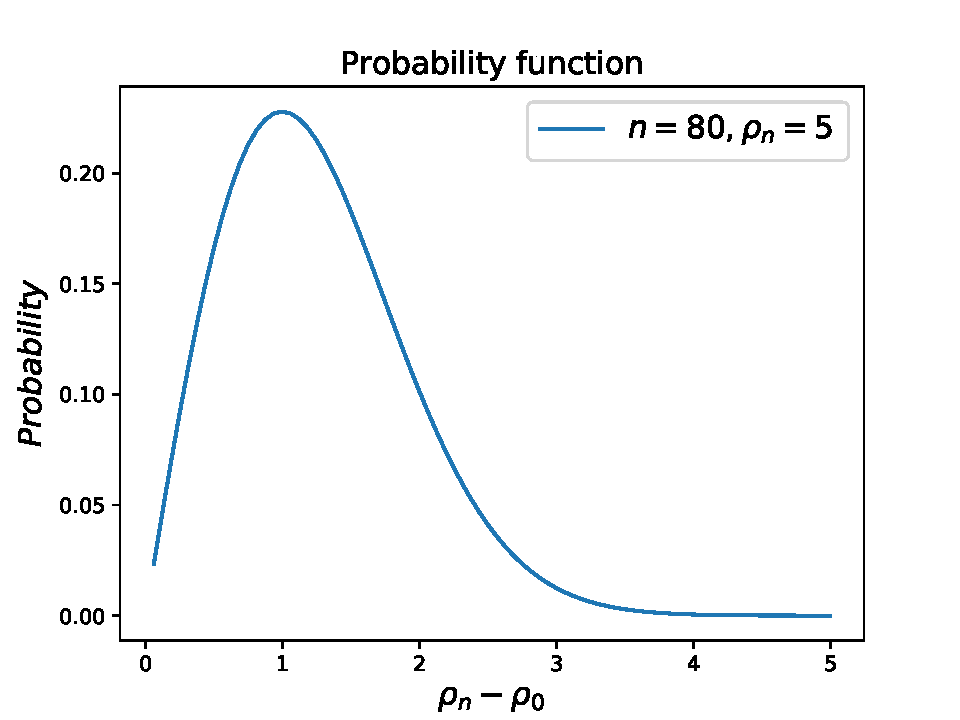
\includegraphics[scale=0.53]{Resolution1_15.pdf}}
}\qquad
\subfloat[Increasing the interval $\rho_{n} = 20$ significantly lowers the resolution of the plot because the number of points per interval decreases.]{{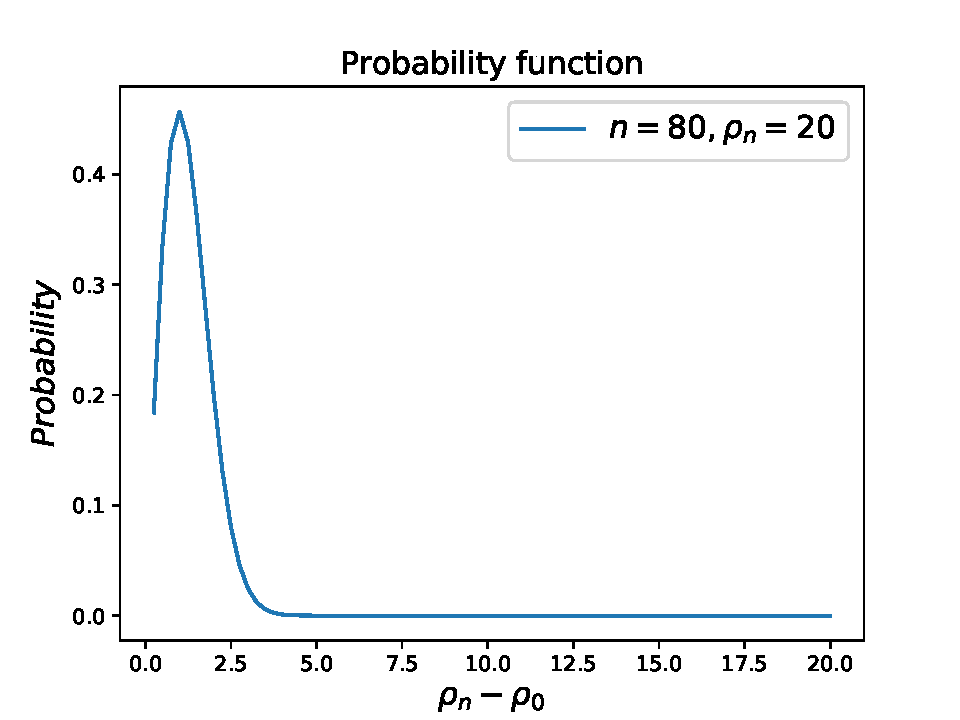
\includegraphics[scale=0.53]{Resolution2_15.pdf}}
}\qquad
\caption{Jacobi's method on a single quantum dot for matrix size $n = 80$ and two different intervals $\rho_n = {5}$ and $\rho_{n} = 20$.}
\label{fig:fig2}
\end{figure}

%\begin{figure}[H]
%\subfloat[tekst.]{{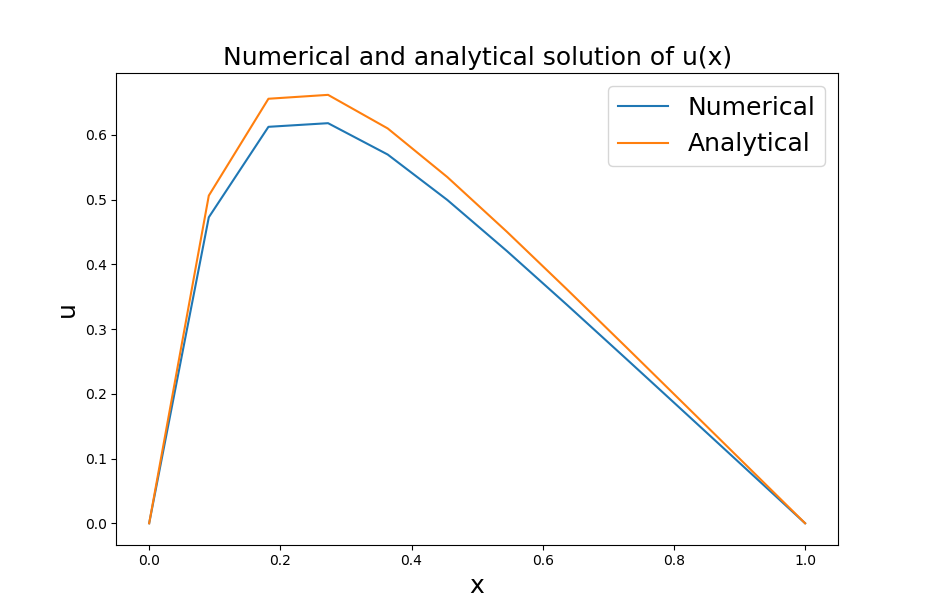
\includegraphics[scale=0.37]{plot1b_n10.png}}%}
%\qquad
%\subfloat[tekst.]{{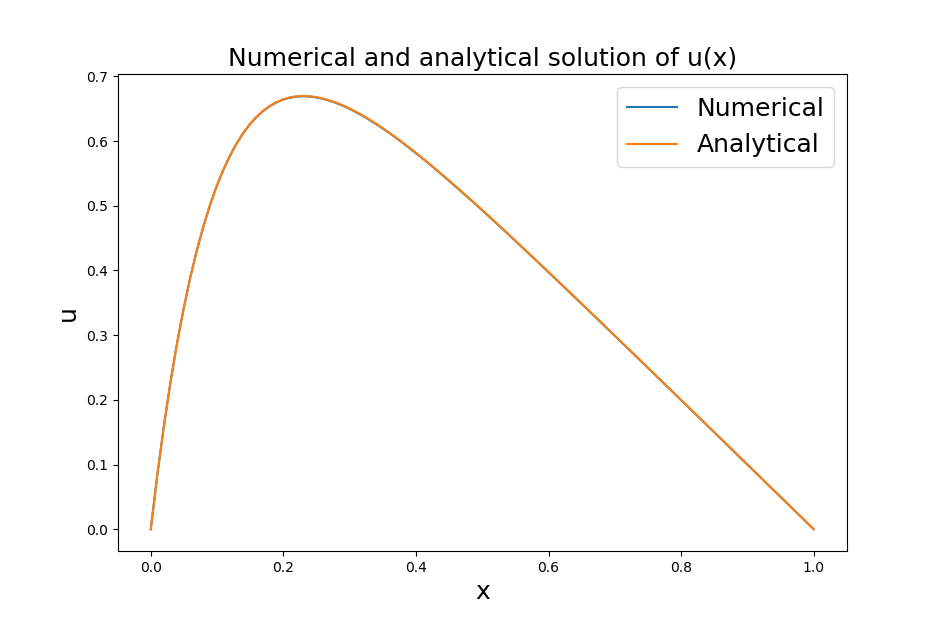
\includegraphics[scale=0.37]{plot1b_n100.png}%}}\qquad
%\subfloat[tekst.]{{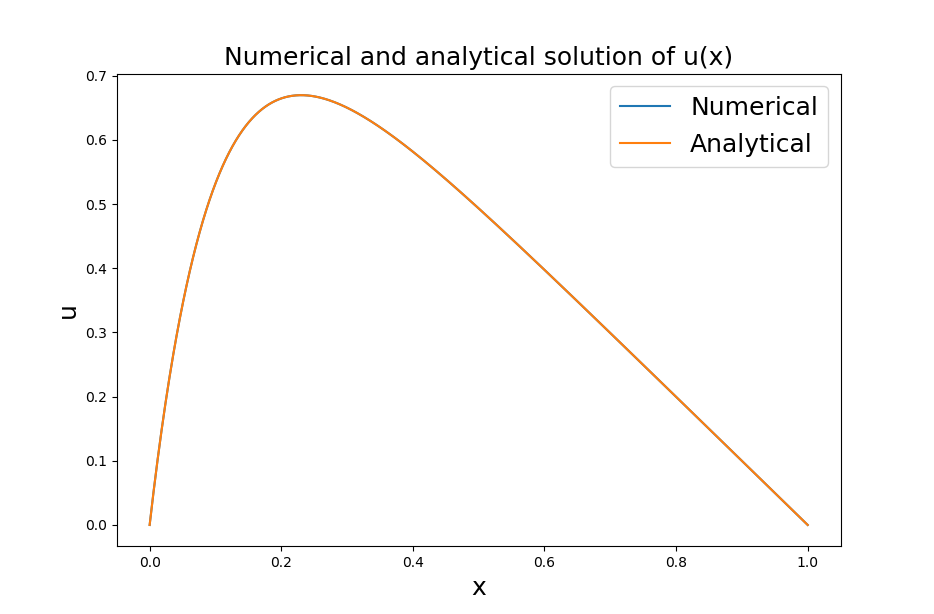
\includegraphics[scale=0.37]{plot1b_n1000.png%}}}
%\caption{tekst.}
%\label{fig:fig1}
%\end{figure}
%

\subsection{Quantum dots, two electrons}

\begin{figure}[H]
\mbox{\epsfig{figure=GSEperOMGr15.pdf,width=\linewidth,clip=}}
\caption{Plot of the ground state energy as function of $\omega_{r}$, it seemingly increases linearly with slope $a = 3.4369$, with error $da = 0.0511$}
\label{fig:fig3}
\end{figure}
%
\begin{deluxetable}{lcc}
%\tablewidth{0pt}
\tablecaption{\label{tab:results3}}
\tablecomments{Table comparing ground stat analytic energy eigenvalues found in \cite{3} and numerical energy eigenvalues, the analytic eigenvalues displayed in the table of the source are halved, $\epsilon ' = 0.6250$, for $\omega_{r} = 0.25$ and $\epsilon ' = 0.1750$ for $\omega_{r} = 0.05$.}
\tablecolumns{4}
\tablehead{$\omega_{r}$ & Analytic $2\epsilon '$ & Numerical $E_{00}$}
\startdata
0.25 & 1.250 & 1.24999 \\
0.05 & 0.350 & 0.349999
\enddata
\end{deluxetable}
%
\begin{figure}[H]
\mbox{\epsfig{figure=ProbfuncperRhons15.pdf,width=\linewidth,clip=}}
\caption{Plot of probability distribution of the two electron quantum dot in a harmonic oscillator potential for different $\omega_{r}$, as well as for no Coulomb interaction. The probability is plotted as a function of the dimensionless relative particle position $\rho = \rho_n - \rho_0$. The maximum value of the $\rho_n$ is an approximation of an infinite value, and is selected as the value where the wave function has vanished}
\label{fig:fig4}
\end{figure}





\section{Conclusions}
\label{sec:conclusions}

\subsection{Jacobi's method}
Utilizing Jacobi's method on scaled differential equations have proven to be a powerful tool for classical and quantum mechanics problems alike. When reviewing numerical accuracy of the method  compared to the analytic results given in \cite{2}, it gives results accurate down to at least 8 significant figures. This result is unique for Toepliz matrices, meaning for other tridiagonal matrices like the ones in the quantum mechanis part of this paper the numerical precision is no longer as high compared to analytical results. However in comparison to other methods it is quite demanding as the number of iterations increases along a quadratic dependency of $n$ [fig: \ref{fig:fig1}], the size of the matrix. In addition the method increases quite fast in CPU-time meaning that the method will not be very versatile if one would need a large $n$. Already at $n = 400$ the CPU time passes $30$ seconds, where Armadillo's method for solving an eigenvalue problem has a CPU time of less than a second.

\subsection{Quantum dots, one electron}


\subsection{Quantum dots, two electrons}

\begin{figure}[H]
\mbox{\epsfig{figure=Omg_r.pdf,width=\linewidth,clip=}}
\caption{Plot of a quadratic potential scaled by $\omega_{r}$ like our harmonic oscillator potential, it is apparent that as $omega_{r}$ increases the potential becomes increasingly confined}
\label{fig:fig5}
\end{figure}


%We have managed to reduce a 3 dimentional two body problem to a analytically solvable problem by changing coordinate system from euclidian to radial, and analyizing CM-system(?)




%\begin{figure}[t]
%
%\mbox{\epsfig{figure=filename.eps,width=\linewidth,clip=}}
%
%\caption{Description of figure -- explain all elements, but do not
%draw conclusions here.}
%\label{fig:figure_label}
%\end{figure}



%\begin{deluxetable}{lccc}
%\tablewidth{0pt}
%\tablecaption{\label{tab:results}}
%\tablecomments{Summary of main results.}
%\tablecolumns{4}
%\tablehead{Column 1  & Column 2 & Column 3 & Column 4}
%\startdata
%Item 1 & Item 2 & Item 3 & Item 4
%\enddata
%\end{deluxetable}




\begin{acknowledgements}
\end{acknowledgements}


\begin{thebibliography}{9}

\bibitem{1}
 Stig-Nicolai Foyn, Christer Dreierstad
\textit{Project 1}

\bibitem{2}
 Morten Hjorth Jensen
\textit{Project 2}
\url{http://compphysics.github.io/ComputationalPhysics/doc/Projects/2018/
Project2/pdf/Project2.pdf} (01.10.18)

\bibitem{3}
 M. Taut
\textit{Two electrons in an external oscillator potential: Particular analytic solutions of a Coulomb correlation problem}
\url{https://journals.aps.org/pra/abstract/10.1103/PhysRevA.48.3561} (01.10.18)

\end{thebibliography}


\end{document}
